\documentclass[10pt,a4paper]{article}
\usepackage[latin5]{inputenc}
\usepackage{amsmath}
\usepackage{cleveref}
\crefname{section}{§}{§§}
\usepackage[a4paper, margin=1.25in]{geometry}
\usepackage{amsfonts}
\usepackage{amssymb}
\usepackage{graphicx}
\usepackage[backend=biber]{biblatex}
\bibliography{Hackathon}
\author{csaaw}
\title{Title!}

\begin{document}
\maketitle

\section*{abstract}

\section{introduction}
\label{sec:intro}

This paper explores the question: how much can the chemical composition of pottery fragments tell us about the evolving connections between settlements in Bronze Age Greece? 




\section{literature review}
\label{sec:litrev}

In this section, two categories of literature are surveyed: (a) theories of Bronze Age trade relevant to the movement of ceramics, and (b) relevant archeometric and modeling methods.

Our dataset includes ceramic shreds from the 7th century BC to the Roman period, but mainly consists of works from the Late Helladic Period - III (LH III, see \cref{fig:timeline} for a chronology)
\cref{fig:seamap} is a map with dashed lines encoded hypotheses about prominent sea routes in the late Bronze Age.  


Maps like \cref{fig:seamap} are of tremendous historical significance if they can be constructed accurately. A common way to map trade is to identify artifacts that have been transported from their location of origin.  How do researchers infer where ceramic objects and shreds originate? 


\newcommand{\foo}{\hspace{-2.3pt}$\bullet$ \hspace{5pt}}
\begin{figure}
\scalebox{1}{
\begin{tabular}{r |@{\foo} l}
 7000 & Beginning of widespread use of pottery in Mediterranean.
Aegina as maritime center\\
3200-2000 & Early Helladic  \\
3200-2500 &  High point of Anatolian trade network \\
2000-2200 & Disruption of trade between Cyclades, Mainland, and Crete. Upheaval in Mainland \\
2000-1550 & Middle Helladic. Protopalatial and Neopalatial buildings in Crete \\
1650-1500 & Late Helladic I / Late Cycladic I / Late Minoan IA \\
1500-1400 & Late Helladic II \\
1400-1300 & Late Helladic III A \\
1300-1200 & Late Helladic III B. High point of Mycenaean influence on trade\\
1200-1050 & Late Helladic III C \\
1050- & End of Bronze Age. Transitional Period: Argos, Asine and Berbati rise to prominence. 

\end{tabular}
}

\caption{Timeline of Events of Interest (all dates B.C.)}

\label{fig:timeline}
\end{figure}

Qualitative methods include categorization by geometric features, and material features. For instance, Davis\cite{davis1979late} classifies pieces from LH I Korakou by shapes, as well as surface and burnishing, measured by the eye against a color chart.  The task is to sort shreds and pieces by style, and also material - these two elements are necessary to differentiate cases where a style travels but pieces are built from local materials. A qualitative study we'll discuss in detail later is that of Rutter\cite{rutter1975ceramic} - he uses the shapes and visible properties of pottery found in Korakou to argue that those pieces were erroneously categorized as Mycenaean. That is: qualitative differences are used to prove a classification claim.  


\begin{figure}
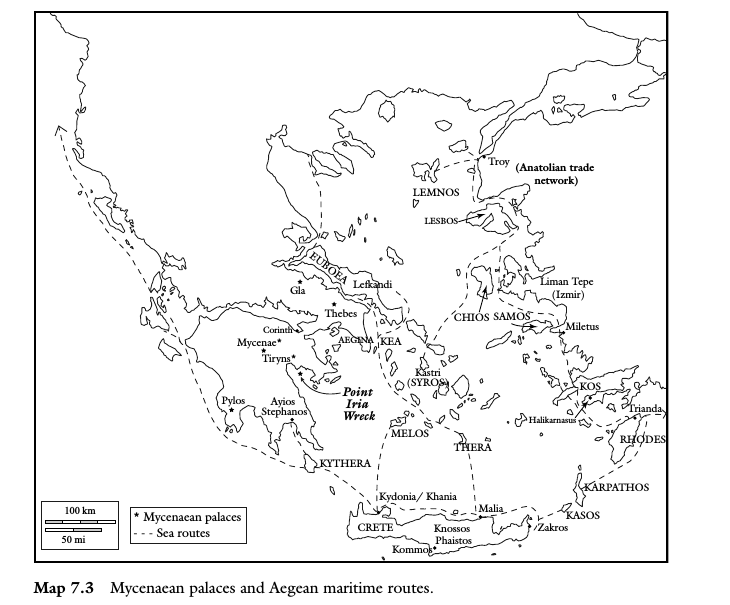
\includegraphics[width=\textwidth]{pottery2.png}
\caption{image from \cite{demand2011mediterranean}}
\label{fig:seamap}
\end{figure}

Quantitative work in classifying pottery mainly uses data from neutron activation analysis or spectral analysis of paints.  This paper uses a neutron activation analysis dataset from the LBNL archeometry archives. The extant work on this dataset (which contains subsections for many geographical areas across the world) has mostly been conducted by Mommsen and colleagues. This work has two main goals: first, to be a proof of concept for quantitative analysis by reproducing known results from limited data, and second, to discover previously unknown connections as a bridge for further inquiry, both qualitative and quantitative.  So for instance, in \cite{mommsen2002complete}, Mommsen et al take their model to succeed by matching existing predictions about early recipe variation in Argolid pottery suggested by Hoffman et al, and by adding new predictions in the case of suggesting a pattern of export from Chania to Cyprus of cream ware.  Grave  et al\cite{grave2014ceramics} follow a similar method of combining the LBNL dataset with other information, also with Cyprus late Helladic wares. 


\begin{figure}
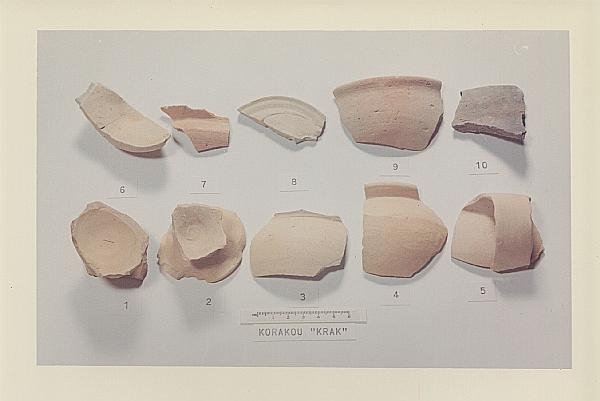
\includegraphics[width=\textwidth]{korakou}
\caption{Example of shreds in the database}
\label{fig:sample}
\end{figure}





\section{method}

\printbibliography

\end{document}
